\subsubsection{Cube ou continuation}
Cet opérateur a été créé pour être une réponse efficace à nos problèmes.
%
Dans notre cas, le graphe à ordonnancer à exactement la même structure que le réservoir que nous souhaitons modéliser.
%
En numérotation naturelle et avec un modèle 3D, une bonne agrégation consiste à agréger toutes les tâches d'un axe qui ont les mêmes coordonnées sur les deux autres axes.
%
Ca correspond à {\em aplatir} notre modèle 3D en un modèle 2D.
%
Par exemple, un cube de 2 éléments de coté, soit 8 tâches, sera transformé en un carré de 2 éléments de coté, soit 4 tâches.

%   (-_-)   %
\begin{figure}[t!]
  \centering
  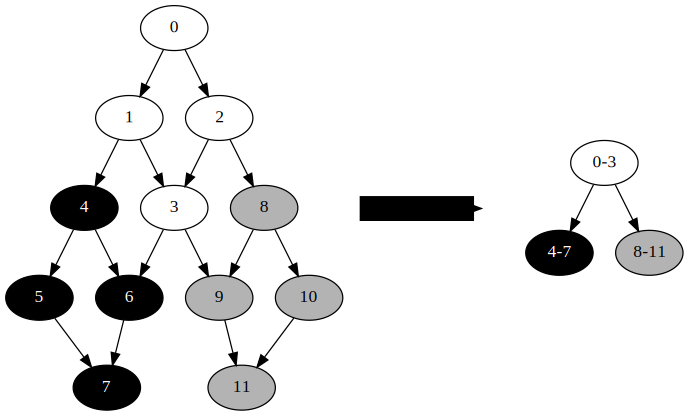
\includegraphics[width=0.8\textwidth]{algo_3}
  \caption{Exemple d'utilisation de l'opérateur C.}
  \label{fig:algo_C}
\end{figure}

Comme pour les autres opérateurs, nous devons vérifier qu'aucun cycle ne sera créé.
%
Pour fonctionner, cet opérateur a besoin que le programmeur attribut un nombre unique à chaque tâche.
%
Dans notre cas on va utiliser la numérotation naturelle.
%
Puis l'opérateur agrégera ensemble les tâches ayant des nombres qui se suivent ainsi qu'une dépendance entre les tâches.

Ajoutons un prédicat à l'algorithme : pour pouvoir utiliser cet algorithme, il faut absolument que pour chaque tâche $i$, le nombre associé à la tâche $i$ soit strictement inférieur aux nombres associés aux successeurs de la tâche $i$.
%
Ce prédicat nous permet de s'assurer qu'aucun cycle ne sera créé.
%
En effet, pour créer un cycle avec cet algorithme, il faudrait
